\chapter{IDEMIX Based Solution}
\section{Introduction}
In this chapter we will provide a solution using IDEMIX based IMS. We will give more details about how this system can be implemented, and how will it behave for the end users.
\section{IDEMIX IMS}
As in previous case we can replace IMS with IDEMIX based IMS in our pseudonymous system. This system will take user credentials and then send an IDEMIX token to the bank. This IDEMIX token contains pseudonym as well as account ID and policy for the user. This IMS can be controlled by a separate identity inside the bank or by a 3rd party.
\begin{figure}[h]
	\centering
	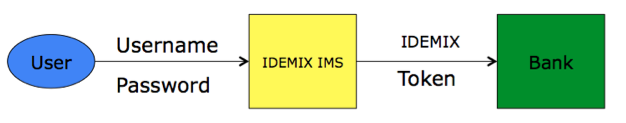
\includegraphics[width=\textwidth]{figures/IDEMIX}
	\caption{Pseudonym System with IDEMIX IMS}
	\label{fig:IDEMIX}
\end{figure}
\section{System Setup}
The system can be setup in 2 ways:
\begin{itemize}
	\item IMS controlled by a separate department at bank.\\
	In this case the bank separate the authentication and service part in 2 different departments internally. Authentication is controlled by IMS which holds the IDEMIX credentials for the user. Service department only gets the IDEMIX token from the authentication department.
	\item IMS controlled by a third party\\
	In this case the bank operates the service part while the authentication part is operated by a trusted third party.
\end{itemize}
In both cases, bank and IMS have to collaborate. Bank have to trust the IMS system that IDEMIX token sent by the the IMS system is correct.
\subsection{Changes on the Bank Side}
In this system, bank needs to behave as an IDEMIX issuer and verifier. It will issue IDEMIX credentials for the users and also will verify the tokens sent by the IMS system. 
\subsection{Information Stored at IMS}
IMS system will behave like user in the IDEMIX system. IMS needs following user information to be stored
\begin{itemize}
	\item User IDEMIX credential
\end{itemize}
Account ID and policy can be stored in encrypted form in the credential itself. This IDEMIX credential for a particular user can be setup in the beginning and then can be used later to create authentication tokens.
\subsection{Changes needed on the User Side}
On user side no changes are needed. User access the system like before. User doesn't need to install any special software or hardware on his side to access the bank services. 
\section{User Creation}
Following are the steps for creation of a new user account in OpenID based system
\begin{itemize}
	\item User goes to bank to open a new account.
	\item User provides his details.
	\item Bank creates user policy and send this information to the IMS system along with other user information as an IDEMIX credential.
	\item IMS system verifies the IDEMIX credential for the user and provides user with credentials to access his account.
	\item User then can login to his account using the credentials.
	\item In case of corporate users, if user is the administrator then he can add more users using a web interface at the bank directly and decide account policies for those users.
\end{itemize}
\section{User Authentication}
Authentication steps are as following in IDEMIX based system
\begin{itemize}
	\item User goes to login page
	\item User provides his username and password
	\item This is sent to IDEMIX IMS which then gets the saved user credential and creates a presentation token with a pseudonym for the bank
	\item Also for escrow purposes the real user identity is also encrypted in the token with the public keys of authorities
	\item Bank receives this presentation token and gets the following information
	\begin{itemize}
		\item Pseudonym
		\item Account ID
		\item Policy
	\end{itemize}
	\item Bank adds this information in a temporary policy database
	\item Bank saves the token for future escrow purposes
	\item User can then access services from the bank using the pseudonym
	\item All user transactions are logged with the pseudonym
\end{itemize}
\section{ID Escrow}
Following are the steps for ID escrow in IDEMIX based system
\begin{itemize}
	\item Authorities come to the bank for transaction data and IDEMIX token.
	\item After verifying, bank gives the transaction data and corresponding IDEMIX token to the authorities.
	\item Authorities then using their key get the real identity of the user from the IDEMIX token.
\end{itemize}
\section{Summary}
This chapter described the IMS system setup using the IDEMIX system. We described how the system will be setup and how it will affect all the parties involved. We will analyze this system later in chapter 8.

